
% 2400 signs per page setup:
\documentclass[a4paper, 12pt]{article}

\usepackage{geometry}
\usepackage{amsmath}
\usepackage{color}
\usepackage{graphicx}
% images alongside text
\usepackage{wrapfig} 
\usepackage{hyperref}
\usepackage[parfill]{parskip}
% blank pages
\usepackage{afterpage} 
% http://ctan.org/pkg/{fancyhdr,graphicx,lastpage}
\usepackage{fancyhdr,graphicx,lastpage}
% get the degree symbol
\usepackage{gensymb} 
% subfigures inside of normal figures
\usepackage{subcaption} 

% Define margins for page setup
\newgeometry{vmargin={30mm}, hmargin={30mm}, tmargin={30mm}, bmargin={30mm}}

\graphicspath{ {./src/} }

% Clear header/footer in favor of the custom header/footer setup
\fancypagestyle{plain}{
  \fancyhf{}                                       
  \fancyhead[L]{Surface-EMG Processing & Classification for Muscle Interfaces}
  \fancyhead[R]{University of Southeren Denmark}
  \fancyfoot[L]{Thomas Alexgaard Jensen (tjens18)}
  \fancyfoot[R]{\thepage\  / \pageref{LastPage}}
}
% Set page style to plain.
\pagestyle{plain} 

% Define Title Page information
\title{Surface-EMG Processing & Classification for Muscle Interfaces}
\author{
\\University of Southeren Denmark
\\
\\Supervisors: 
\\Poramate Manoonpong (poma@mmmi.sdu.dk)
\\Xiaofeng Xiong (xizi@mmmi.sdu.dk)
}

\date{Date: }

% norm symbols for math
\newcommand{\norm}[1]{\lvert #1 \rvert}

% Explanation setup, used for specific words explanation
\newcommand{\explanation}[2]{
\textit{#1: }{#2.}
}

\begin{document}

\maketitle
\newpage

\documentclass[../main.tex]{subfiles}
\graphicspath{{\subfix{../src/}}}


\begin{document}
\section*{Abstract}

% Introduction of problem
The human upper-limbs are some of the most important appendages of the human body.
The upper limbs of a human allows for interaction and manipulation of the environment, and acts as a crucial part of a functioning human body.
% Why we need to solve this problem
The loss of an upper limb, either congential or traumatic severely reduces a person's ability to interact with- and perform simple day-to-day tasks in the enviromnent required for basic human living.
% Introduction to existing solutions and their flaws
This is a major problem for the amputee, and can only be partially solved by rehabilitation using a crude prosthetic device, designed to provide a interface between a mechanical or robotic appendage, and the remaining appendage section of the amputee.
These prosthetics often only allow for a small degree of controllability through a limited interface at the attachment point of the prosthetic.
This often causes the amputee to neglect the rehabilitation and usage of the prosthetic, by choosing to reserve it for limited use, or reject it alltogetther.
Amputees not choosing to make use of a prosthetic device, often cause overuse of their remaining limbs.
% This thesis researches.... Intro to my work
This thesis aims to decrease the gap between existing prosthetic devices and their real-life counterpars, with the purpose of increasing controllability and interactability for the amputee, and by doing so, decreasing the amount of amputees choosing to reject their prosthetic device. 
This thesis researches different control methods of of a prosthetic device, with a focus on processing and interpreting sEMG data recorded from the upper appendage and the upper body.
Furthermore, this thesis prposes an anatomically correct simulated prosthetic hand, designed to visualize and test control methods of a prosthetic device.
Lastly, this thesis researches and compares different methods of Machine Learning and Artificial Intelligence in order to convert sEMG data into a controllable output for a prosthetic device.
% This thesis proposes... outcome of my work
This thesis proposes the use of feature-based Linear Discriminant Analysis intent classification, and the usage of a 4-layer Recurrent Neural Network to predict the joint movements of the hand.


\end{document}

\documentclass[../main.tex]{subfiles}
\graphicspath{{\subfix{../src/}}}


\begin{document}

\section{Acknowlegdements}

Hello, here is some text without a meaning...

\end{document}

\include{content/terminology.tex}

\tableofcontents
\newpage

%TODO: Add figures to table
%\tableoffigures
%\newpage

\documentclass[../main.tex]{subfiles}
\graphicspath{{\subfix{../src/}}}


\begin{document}

\section{Introduction}

The human hand is one of the most important factors of the human identity.
The hand allows a person  to perform complex muscolatory combinations to interact with the surrounding world, express complex emotions during speech, and aid in defining a person's individuality and personalty \cite{???}.
% TODO: cite "Grasping the Importance of Our Hands"
The hands are controlled by a complex combination on precise muscles designed to perform gentle, precise control of the fingers.
This allows a person to grasp objects in many different ways, perform complex tasks such as writing, playing musical instruments, or even constructing a house.
The hand also acts like a sensory device allowing us to perform precise observations through feeling and touch.
This allows a person to understand the environment without seeing it, the hand is able to sensor heat/cold, create complex understanding of geometries and texture through touch and manipulation.

Missing limbs, either \gls{congential} or \gls{traumatic} amputation severely reduces a person's ability to interact with- / understand the world, express themselves and perform simple day-to-day tasks.
In order to alleviate some of the drawbacks of missing a limb, amputees are often able to aquire a prosthetic replacement of their lost limb.
The aquired prosthetic tries to imitate the movements of the lost limb, through muscle-activated interfaces, that is then used to control the movements of the prosthetic. 
In the case of hand prosthetics, the prosthetic allows the user to perform simple, day-to-day tasks, and is able to alleviate some of the stress caused to the non-amputated hand through overusage.
%TODO: Refrence here

%TODO: Get a cool image of a prosthetics user
\begin{figure}[h]
\begin{center}
\includegraphics[width=0.8\textwidth]{example-image-a}
\caption{Example figure text}
\label{fig:template}
\end{center}
\end{figure}

This thesis aims to summarize, and elaborate on current state-of-the-art research and products in the field of prostetics devices, and products the control of prosthetics and the existing limitations of these state-of-the-art products. 

This thesis aims to contribute to the world of prosthetics control, by researching effective methods of collecting sensory data from the lower-/upper-arm, and by doing so, creating an state-of-the-art Artificial Intelligence (AI) based controller, that is able to imitate the intent and movements or a real hand.
And by doing so, by improving sEMG controller design to increase functionality and the controllable DoF of the prosthetic, to provide a more true-to-life experience to the prosthetics user, and thus reduce the amount of patients that disregard prosthetics.

This thesis also aims to explore efficient methods of designing a network to identify lower-/upper-arm muscolatory intent, with the purpose of controlling a simulated prosthetics device, and by doing so, increase the controllable Degree-of-Freedom for the prostetics user.

\end{document}

\documentclass[../main.tex]{subfiles}
\graphicspath{{\subfix{../src/}}}


\begin{document}
\section{Problem Specification}

There is a large need for new technology that improves the effectiveness and ergonomics of human hand prosthetics.

Current state-of-the-art products on the market exhibits a severe reduction of controllable Degree of Freedom (Dof) compared to their biological counterparts.
These products often rely on simple, grasp control based on 2 or more \gls{sEMG} interfaces, to classify ``open/close'' signals for the control scheme.
The prosthetics user is then manually required to change grip control-scheme, creating very crude control dynamics that is very different from biological hand-control.
A in-debth explanation of ``open/close'' control can be seen in section \ref{???}
%TODO: This sounds weird, integrate a simple controller therory here, and why it is so crude, then refrence it in state-of-the-art
%TODO: Create refrence
This is a great pitfall in the field of Research and Creation of prosthetics, as unsatisfactory function of prosthetics lead to amputees, that exhibit a great deal of stress douring the rehabilitation process.

%TODO: Refrence for this!
This can cause the patient to repel the rehabilitation process and the prosthetic all-together.
The repelling of the prostetic increase in the cases of the most severe cases of amputation, where the largest amount of control muscles are lost.
These amputations are often located further up the limbs, where the loss of mobility and controllability are greatest.
The amount of muscles leftover from amputation also dicates the type of prosthetic a patient is able to recieve.
%TODO: Refrence for this!
Patients of lower-arm amputation has less control over their prosthetic than patients of hand amputation, due to the loss of the muscles in the lower-arm.
The loss of control increases as the amputation severity increases, and this is a problem in prosthetics design because it is impossible to create a standardized controller that suits most patient's needs.

State-of-the-art commercial prosthetics further decrease the controllable DoF in order to increase robustness of the control experience, this is further elaborated upon in \ref{sec:stateoftheart}.
%TODO: Create refrence for state-of-the-art

\subsection{Motivation}

The main goal of this thesis is to provide a meaningful contribution to the world of prosthetics design and control.
In order to confine the workload done in this thesis, a set of development goals has been made:

%TODO: Refer to these in the report! make it the key motivations for all my choises.
\begin{enumerate}
\item Create a software-based, biology-inspired, anatomically realistic simulation of a humanoid lower-arm/hand that is able to imitate the movements of the humanoid limb.
\item Make the prosthetics simulation controllable from a widely-used robotics-software.
\item Design a sEMG muscle pre-prossesing pipeline for a prosthetics controller. 
\item Design a state-of-the-art prosthetics controller based on AI, to control a simulated prosthetics device.
\item Create a custom dataset to train AI based controllers for prosthetics.
\item Test and Validate the created prosthetics controller against state-of-the-art methods.
\end{enumerate}
%TODO: This needs


\end{document}

\documentclass[../main.tex]{subfiles}
\graphicspath{{\subfix{../src/}}}


\begin{document}

\section{Literature Review}

As sensors capability for for biological sensoring increases in state-of-the-art prosthetics development and research, there becomes a larger need for translating sensor data into usable input data for prosthetics controllers.
A lot of reserach has been done in this area, this research elaborates on different Machine learning or AI-based methods of understanding muscle-based sensor data.
The pipeline for converting EMG sensor data to usable input data often contains a pre-processing step, where data is de-noisified, and cleaned of potential errors.
The pre-processing step can also contain feature extraction such as ...
%TODO: Mention some example stuff like extracting features of raw data, i think RMS, and other spaces.
The pre-processing step is then followed by a processing step, this step encompasses the use of a Machine-learning algorithm or a Neural Network, designed to either Classify a grip type, or Regress the angle of the joints.
After Classification or Regression a post-processing step can be added where the actual kinematic data is created, and used as input to the prosthetic controller. 
Popular methods of processing EMG signals will be researched, and elaborated upon, with the aim of identifying robust, effective and implementable methodologies.
% that can be tested in the context of the thesis, and the dataset i create...
%TODO: Can i do something like this?


\subsection{Introduction to Literature}
%TODO: Maybe this text fits better elsewhere?

Human Machine Interfaces (HMI), are control systems that enables humans to interact and control a mechanical or robotic system.
%Prosthetics have been developed to aid human behaviour 
%TODO: Somehow say that prosthetics are found en ancient egypt etc.
%TODO: Make proper citation!
As explained in the paper \cite{Tech2015}, researchers and prostecisists have been developing mechanical prosthetics for many years.
One example of such devices would be the ankle-foot-orthoses, a support device strapped to the angle, used to relieably adjust the pressure applied by the body while walking, to help impared individuals with walking in a more natural way.
\cite{Tech2015} proposes that EMG signal based control research are a ongoing topic in rehabilitation and prosthetics.
Generally, EMG is an experiment-based method of evaluating and recording electrical signals from muscles.
Specifically, EMG signals eminate from the exiciability of muscle fibers through neural control, causing action potentials that cause depolarization and repolarization of the muscle membrane.
These polaziration changes can be detected using EMG sensors, either through non-invasive or invasive techniques.
Invasive EMG signal recording requires the use of a penetrating needle electrode to be placed in the muscle tissue, this method reduces the signal-to-noise ratio (SNR) but can be a cause of discomfort and infection.
As an alternative, non invasive EMG sensors, placed at the surface of the skin are called sEMG sensors, they provide much less discomfort and propose no risk of infection to the amputee, at the cost of having an increased SNR. 
\cite{Tech2015} explains that the muscle fiber membrane has a resting potential of $-90$ to $-90 mV$ when resting. The paper also explains that the amplitude of sEMG signals have a voltage range from $0$ to $10 mV$, and a frequency range from $10$ to $500 Hz$.

\subsection{Noise in EMG signals}

The paper \cite{Tech2015} poposes different noise types that contaminates EMG signals, these noises are defined as electrical signals that are not part of the decired EMG signal.
%TODO: maybe find the paper that Tech2015 refers to and insert it here for variety its number [8]
The different noise types found in EMG signals are
\begin{itemize}
\item Inherent Noise in Electronics Equipment,
\item Ambient Noise,
\item Motion Artifacts,
\item Inherent Signal Instability,
\item Electrocardiographic (ECG) Artifacts,
\item \& Cross Talking.
\end{itemize}

%TODO: Adjust the texts for noise signals to be coherent to be coherent
%These noise types are all
\textbf{Noise in Electronics Equipment} exists in all electronic devices, this noise has been proved to be reduced by using electrodes made of silver.
%TODO: ref on this!
\textbf{Motion Artifacts} affects EMG signals when the skin and electrodes move in relation to the movement of the underlying muscle.
This can cause artifacts due to inconsistent displacement.
%the length of the muscle decreases when muscles are activated. Muscle, skin and electrodes also move in relation to each other. 
\textbf{Inherent Signal Instability}, The amplitude of EMG signals are quasi-random. Frequency components less than 20 Hz are unstable and affected by firing rate of the motor units. This range is considered unwanted noise. Muscles change based on their active motor units, therefore the EMG signal changes too.
\textbf{ECG Artifacts} is the electrical activity of the human heart is a huge interference component of EMG signals recorded from the Shoulder Girdle (Shoulder muscle groups).
%this is called ECG Artifacts.
%this contaminated EMG signals, especially "trunk EMG"
It is very hard to remove ECG artifacts from EMG signals, due to their relative charactaristics in the frequency spectrum!
% TODO trunk muscles EMG
\textbf{Cross Talk} is undecired EMG signals from muscle groups not commonly monitored. i guess its a form of EMG leak from undecired muscles.

%People with lower-leg amputation able to recive mechanical prosthetics. The need to introduce robotic prosthetics in this area  Due to the  limited mechanical movement and control of the human ankle/foot, p
%TODO: Somehow incorporate this? if you do, ref on this!

%Use-Case for 
\subsection{sEMG Sensors for Prosthetics}

The usage of sEMG sensors propose a lot of obstacles because of noise, but that does not stop sEMG sensors from being part of the state-of-the-art research in prosthetics.
In the paper \cite{KeunTaeKim2021} proposes that the usage of sEMG sensors are of great importance in upper-limb classification for prosthetics devices.
The paper uses sEMG sensors to classify reaching-to-grasping tasks using  a Convolutional Neural Network (CNN) after pre-processing the signal with Principal Component Analysis (PCA) to reduce noise.
The processing combination method of PCA-CNN proved to show higher accuracy than Machine Learning methods, such as Support Vector Machine (SVM) with an accuracy of $70.1 \pm 9.8\%$ based on 9 subjects.
%TODO: When i get results, precent it like a median + - percentage variation for my subjects! makes it sound statistical and cool..
The paper proposes that the sEMG sensors are placed on the upper-body in combination with the upper-arm for grasping intention classification, specifically, the muscles \textit{Pectoralis}, \textit{Trapezius}, \textit{Latissimus Dorsi} \& the \textit{Biceps/Triceps}, see section \ref{sec:muscleplacements} for placements.
%TODO: We need a section with all the muscles i intend to classify!
In \cite{KeunTaeKim2021}, the \textit{Southhampton Hand Assessment Procedures (SHAP)} \cite{shap} was used to create a dataset.
SHAP is designed for the assessment of musculoskeletal and neurological conditions, and can be used to test the effectiveness of prosthetics.
%TODO: This is formulated wierdly..
%TODO: explain that you USE the KeunTaeKim2021 Network as a baseline for one of your own networks!

Another paper that proposes the usage of sEMG sensors for prosthetics is \cite{Zhaolong2021}.
The paper
The paper proposes the usage of different sEMG devices, two of those are the wearable product ``Myo Armband'', \cite{myo} a discontinued sEMG product consisting of 8 sensors that can be placed below the elow joint, and the ``Delsys Trigno'' \cite{trigno}, a set of individual sEMG sensors that can be worn and record most muscle groups.
\cite{Zhaolong2021} proposes the pre-processing of the sEMG data using a Notch filter of 50Hz.
Furthermore, the target angles obtained as ground truth targets were reduced in dimensions through PCA, thus having the 6 dominant PC's be the targets.
Then, using an ``Inverse PCA algorithm'', they compute the final control output for the prosthetic.
In order to process the sEMG data, \cite{Zhaolong2021} proposes the use of a time window of $200ms$, with feature extraction for root mean square (RMS) \& zero crossing (ZC).
%TODO: If i use this myself, i need to write the equations from this paper!
The extracted features were used as input to a nonlinear autoregressive exogeneous (NARX) network, a fully-connected multilayer-perceptron (MLP) network combined with a recurrent neural network (RNN). 
% once the report is done, check up on abbrevations etc and make sure things are abbrevated once and then used!
% TODO: Maybe give a link for further explanation?
%TODO: Zhaolong2021 -> their results are so good i need to try their method!

\subsection{Adaptive Grasping Methods}
%\subsection{Adaptive grasping methods of sEMG based prosthetics}
%\subsection{Adaptiveness of sEMG based prosthetics}
%TODO: Maybe section names should relate more directly to the explained papers?
Most state-of-the-art methodologies consist of using sEMG data to predict grasp type classification or joint angle regression.
The paper \cite{Yuki2023} proposes that this method becomes a burden for the HMI user, as the severity of the amputation increases and the loss of muscle recording arears become greater.
\cite{Yuki2023} takes inspiration from evolutionary robotics, and propses the use of evolutionary computation to predict stable grasping methods based on touch sensor input.
This is done by having a mapping between the touch sensor input of the fingers and the motorcontrol of the joints.
\cite{Yuki2023} uses a simulation to train a RNN network, this RNN takes sEMG sensor data, Touch sensor data, distance to the object \& object height into account.
It is possible to compute distance to / height of object because grasping and training is done entirely in simulation, using a simulated target object, but that the method used would be realiseable for prosthetics. 
The paper concludes that alongside sEMG sensors, touch sensors could be used to appropiate joint motion could be predicted using contact states between hand and object.

The paper \cite{YanchaoWang2022} proposes a passive solution to adaptiveness when grasping.
Their method uses an underactuated, compliant linkage mechanism, where the joint rotation of the finger joints can be driven by a single motor.
This allows the fingers to not rely on touch sensors, as the method in \cite{Yuki2023} does.
\cite{YanchaoWang2022} proposes the use of a sliding window with a size of $250ms$.
The window is then processed using feature extraction of integral myoelectric value (iEMG), RMS. mean absolute value (MAV) \& ZC with a threshhold to eliminate low signal fluctuation from noise.
The extracted features are used for linear discriminanr analysis (LDA) to classify grasping intent. 
The paper proposes that LDA showed the highest accuracy out of different Machine Learning methods.
%TODO: Is last sentence vague?





\subsection{sEMG Classification}
%TODO: Come back to Tech2015 and go over some classification stuff.

\subsection{Alternatives to sEMG sensors}
% Explain Brain based systems, nerve based systems, and sEMG systems

\subsection{General Overview of Different Dreas of sEMG Processing}

% refer to Tech2015
% refer to Batzinaulis2018

\subsubsection{General Processing choises for muscle data}
% Jarque2019

\subsection{Regression or Classification}

% Processing methods for both Regression and Classification, get some comparable data to look at.

\subsection{State of the Art Methods}

% here i want to list a set of state of the art methods and their goals, as a appetizer to what
% i want to do..

%TODO: Check out all the papers on your phone and see if they can be used.

\end{document}

\documentclass[../main.tex]{subfiles}
\graphicspath{{\subfix{../src/}}}


\begin{document}
\section{Methodology}

\subsection{Dataset Creation}

In order to train a simulated hand prosthetic, a sofisticated dataset containing the measured relation between muscle activity and the finger placements is needed.
The paper \cite{KeunTaeKim2021} proposes the SHAP procedure \cite{shap} as its main method of dataset creation.
An alternative would be the Sollerman test \cite{sollerman} as both procedures are used in assessing the function and moveability of the human hand.
By analyzing the most important gripping motions in both tests, it should be possible to denote a suitable set of grips that the dataset should contain.
The sollerman grip types are ranked based on their usage percentage in activities of daily living.
The most used grip types according to sollerman are the \textit{Pulp pinch}, \textit{Lateral pinch}, \textit{Five-Finger pinch} \& \textit{Diagonal Volar grip (Power grip)}, see \cite{sollerman} for further details.
SHAP also proposes a set of grip types that are used in day-to-day tasks, these are \textit{Spherical grip}, \textit{Tripod pinch}, \textit{Power grip} \& \textit{Lateral pinch}.

In order to create a dataset mimics the movements of day-to-day tasks, the most important grips from \cite{sollerman} \& \cite{shap} has been chosen.
The grip types that needs to be part of the dataset and their usage descriptions can be seen in table \ref{tab:grips}.

\begin{table}[h]
\begin{center}
\begin{tabular}{ |l|l| } 
 \hline
 Grip Type & Finger Usage Description \\ 
 \hline
 Pulp pinch & Between thumb, index and middle finger \\ 
 Lateral pinch & Between thumb \& side of index finger \\ 
 Five-Finger pinch & Between thumb, and all four fingers \\ 
 Power grip & Between thumb, and all four fingers with contact to palm \\ 
 \hline
\end{tabular}
\caption{The most used hand grips in day-to-day tasks based on \cite{sollerman} \& \cite{shap}.}
\label{tab:grips}
\end{center}
\end{table}

The chosen grips are chosen as a basis for the creation of a dataset. creating 


\subsubsection{Existing datasets}

In addition to creating a specific dataset for this thesis, it would be intresting to compare with an existing state-of-the-art dataset.
The paper \cite{jarque2019} proposes the use of their dataset \cite{kinmusdataset}.


%The recording of the dataset is done using the software explained in section \ref{sec:software}, namely Motive \cite{motive} \& EMGworks \cite{emgworks}.
%TODO: Present more formally and mention company names.

\subsubsection{Motion Capture Glove}

In order to get precise recordings of the motion of the hand and fingers, using Motive \cite{motive}, flourecent 3D markers were placed on a glove.
The pattern of the marker positions were carefully closen in order to calculate the angles of the individual finger bones.
The precise positions of the 3D markers on the recorder glove can be seen in figure \ref{fig:glove}.

\begin{figure}[h]
\begin{center}
\includegraphics[width=0.8\textwidth]{example-image-a}
\caption{Example figure text}
\label{fig:glove}
\end{center}
\end{figure}

\subsubsection{Sensor Locations etc.}

The muscle recording sensors are located along the muscles of the forearm, the exact positions can be seen in figure \ref{fig:musclesensors}.

\begin{figure}[h]
\begin{center}
\includegraphics[width=0.8\textwidth]{example-image-a}
\caption{Example figure text}
\label{fig:musclesensors}
\end{center}
\end{figure}

\subsubsection{Trial/motion overview}

\subsection{Design of a Simulated Prosthetic Hand}

In order to design a state-of-the-art simulated prosthetic hand, a number of anatomical design choises needs to be considered.
This thesis tries to create the most anatomically-correct hand simulation available, this will hopefully have a number of positive effects on prosthetics research.
By having access to an advanced simulation, it would in turn be able to test and visualize more advanced movement controllers that can facilitate more DoF than current commercial prosthetics. 
By creating an anatomically correct prosthetic hand simulation, it is hoped that prosthetics users can have more advanced rehabilitation, and learn to have more natual control of their prosthetics. This would create a more natual usage experience, and decrease the percentage of users that reject the usage of their prosthetic alltogether.

A set of requirements The simulated anatomically correct hand should be determined in order to create a state-of-the-art prosthetics simulation.

The simulated prosthetic should:

\begin{enumerate}
\item Facilitate the same DoF as an anatomically correct hand.
\item Have porpotions that closely resemble that of an anatomically correct hand.
\item Be simulated and be controllable in a commonly used robotics software to increase accesability for researchers.
\end{enumerate}


\subsubsection{Brief of used Software}
\label{sec:software}

Coppeliasim see \cite{coppeliasim}.
%TODO: only for test

\subsubsection{Anatomy}
\label{sec:anatomy}

The hand is an anatomically-complex appendage designed to facilitate a large amount of control in different usage scenarios.
The hand consists of 27 bones, 14 of these are called phalnages, and make up the 4 fingers and the thumb. These bones, alongside a complex set of ??? muscles facilitates 24 DoF (Not counting Translation of the entire hand).
%TODO: How many muscles in the hand / forearm?

The individual finger consists of 3 bones called \gls{phalanges}, arranged linearly from the palm of the hand.
The 3 finger bones are called the proximal phalange, middle phalange and distal phalange.
The joints between the phalanges are able to do \gls{flexion/extension} movement, while the base of the finger is further able to do \gls{abduction/adduction} movement.

%TODO: Muscles of the hand: https://www.assh.org/handcare/safety/muscles
%TODO: Bones of the hand: https://www.bidneedham.org/departments/orthopaedics/hand-program/anatomy-hand-and-wrist

\subsubsection{Simulated Hand Articulation design}

%TODO: see Yuki2023 (page 11) for how to properly show the dimensions of my hand!

In order to translate the biology and anatomy of a real hand into an robotics simulation, we start by denoting the relative lengths of the wrist bones and phalnages by refrence, as can be seen in figure \ref{fig:handref}.

%TODO: IMAGE HERE OF HAND OR XRAY
\begin{figure}[h]
\begin{center}
\includegraphics[width=0.8\textwidth]{example-image-a}
\caption{Example figure text}
\label{fig:handref}
\end{center}
\end{figure}


The porpotions of the refrence is used to denote the bone lengths for the model.
The model is implemented in Coppeliasim \ref{???}, The model is created in a hierachy, the bones are created with cylinders and the joints are created using 1 DoF Revolute joints.
% Ref coppeliasim
As specified in section \ref{sec:anatomy}, some joints of the human hand facilitates 2 DoF of rotation.
This is needed in order for the wrist and finger base joints to be able to do \gls{abduction/adduction}.
To simulate this, two 1 DoF revolute joints were placed in series, thus allowing 2 DoF.

\subsection{Implementation}

Based on the literature review in Section \label{sec:literature}, it becomes apparent that there exists a standard pipeline for translating sEMG recordings into predicted motorcontrol for a prosthetic.




\subsubsection{Data Pre-Processing}
\subsubsection{Network Design}
\subsubsection{Software Hand Design}

\end{document}

\documentclass[../main.tex]{subfiles}
\graphicspath{{\subfix{../src/}}}

\begin{document}

%\subsubsection{Machine-Learning Designs}

%TODO: Some introduction and explanation of feature extraction, what types and papers that uses these.
%TODO: Some introduction and explanation of SVM and LDA types of networks.
%TODO: Go back and see what papers uses these.

%\subsection{Software Hand Design}

%\section{Tests \& Results}

\section{Datasets}

\subsection{Recording of a Dataset}

The created capture glove for the Motive motion capture system and the sEMG sensors from the Delsys Trigno setup is placed on the target, with the sEMG sensors following the setup in \ref{tab:muscletargets}.
The setup can be seen in Figure \ref{fig:musclesensorsonarm}.
Objects of different sizes and weights is placed in front of the target for gripping. 
This is done so that the chosen gripping sequence and environment is highly dynamic, and ideal for creating regression models.

\begin{figure}[H]
\begin{center}
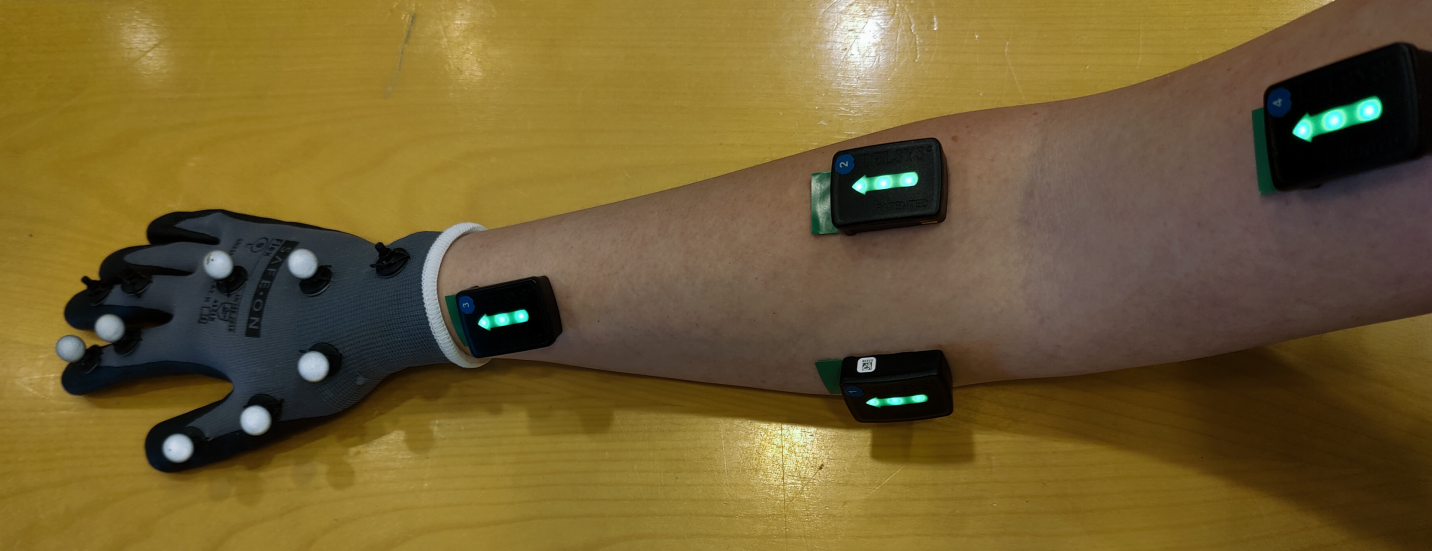
\includegraphics[width=0.99\textwidth]{sensors_on_arms_cropped.png}
\caption{Capture glove and sEMG sensors placed on the recording target. The sEMG sensors are located based on the muscles from table \ref{tab:muscletargets}.}
\label{fig:musclesensorsonarm}
\end{center}
\end{figure}

As explained in section \ref{sec:motiveproblems}, creation of a custom dataset to train and test models on proved to be difficult.
The dataset created using the Motive capture software in section \ref{sec:motiveglove} is not very large, and has no labeling for classification.
Because of this, the dataset is not suitable for training in any of the methods.

\subsection{Labeling of Motive capture data}
%\subsubsection{Cleaning of Motive Capture Data}
\subsubsection{Implementation}
\label{sec:motivecleaning}
%\subsubsection{Reduction of Tracking Software Problems}

%TODO: This section could be expanded and images could be included.
%TODO: HERE I NEED TO GO ALL IN ON DATA CLEANING

%In order to fix some of the problems, caused by the setup, software was written.
%TODO: shitty starter
The large amount of problems observed using the Motive motion tracking software makes it impossible to use the tracking output as training data.
Markers are not tracked correctly and new labels are created every time tracking fails, this can be seen in Figure \ref{fig:motivelabels}.

\begin{figure}[H]
    \centering
    \begin{subfigure}[b]{0.49\textwidth}
        \centering
        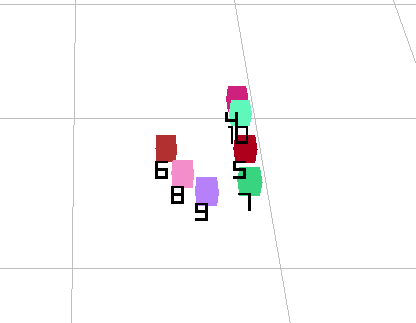
\includegraphics[width=\textwidth]{motivemarkers1.png}
    \end{subfigure}
    \hfill
    \centering
    \begin{subfigure}[b]{0.49\textwidth}
        \centering
        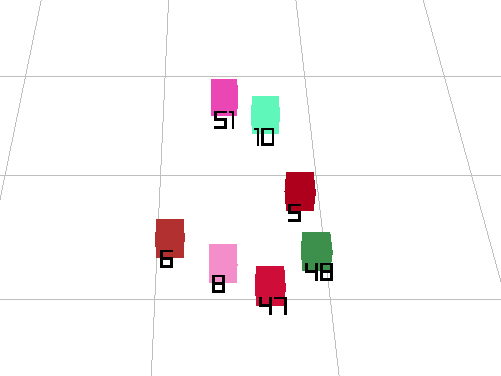
\includegraphics[width=\textwidth]{motivemarkers2.png}
    \end{subfigure}
    \hfill
    \begin{subfigure}[b]{0.49\textwidth}
        \centering
        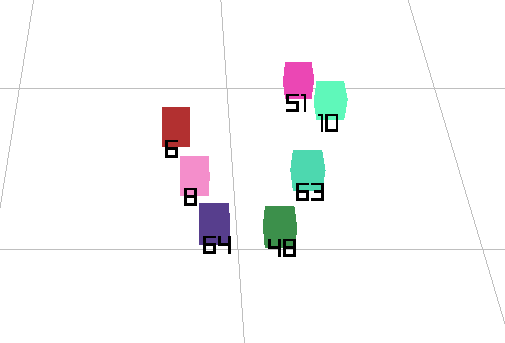
\includegraphics[width=\textwidth]{motivemarkers3.png}
    \end{subfigure}
    \hfill
    \begin{subfigure}[b]{0.49\textwidth}
        \centering
        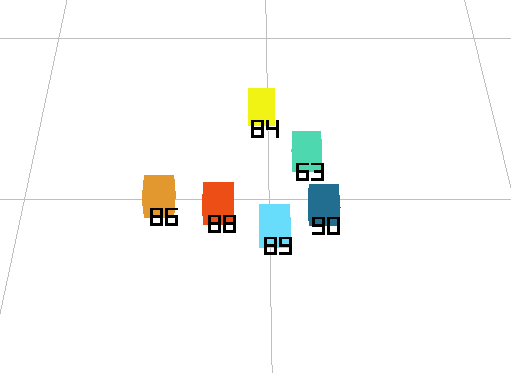
\includegraphics[width=\textwidth]{motivemarkers4.png}
    \end{subfigure}
    \caption{Motive tracking labels changes over time, in this case, the markers changed to new labels at $\sim 2$, $7$, $11$ \& $14$ seconds into the recording, with smaller changes throughout.}
    \label{fig:motivelabels}
\end{figure}

As can be seen in the figure, a recording of 15 seconds creates $\sim 100$ individual labels.
This causes great problems as it becomes impossible to relate one marker to another, and extract the kinematic data for training a model.
The problem requires the user to manually remove and combine labeled marker sections into larger labeled sections, in order to eliminate all changing labels on the tracked markers.
A feature designed to match up mislabeled markers and optimizing the movement paths of markers exists in Motive, but it did not fix the stated problems.
In order to fix this problem and because of a lack of functionality in Motive, two software solutions is created.
Rendering and replaying of the 3D markers in real-time, with their associated labels is handled in one of the created software solutions.
Furthermore, the second software was designed to remove, merge and sub-sample 3D marker output files from Motive.

\subsubsection{Evaluation}

These software solutions are designed to work simultaneously, and is effective at cleaning the labels.
The main problem is that this cleaning of 3D marker labels is a time consuming process, and results in not being able to use the recorded dataset for training a model.
The software created to fix unreliable labeling of markers in the tracking data can be seen in appendix \ref{appendix:motivefixing}.

\subsection{Filtering of Delsys Trigno muscle recordings}

\subsubsection{Implementation}

Based on the literature review in Section \ref{sec:literature}, it becomes apparent that there exists a standard pipeline for translating sEMG recordings into predicted motor control for a prosthetic.
Raw sEMG data contains a lot of unwanted noise as explained in section \ref{sec:noise}.
Some of the noise can be can be removed through signal processing using analog filters.
Different filter types exists, and different filters are used to remove a specific frequency in the data. 
State-of-the-Art papers use a lot of different methods to reduce noise in sEMG data.
The paper \cite{multdof} proposes the use of a $50Hz$ Notch filter, while papers \cite{graspintent} \& \cite{ashirbad2022} respectively chooses a $20Hz$ cutoff Buttersworth filter \& a $10-500Hz$  Buttersworth band-pass filter, lastly the paper proposes a $60Hz$ notch filter in order to remove power-line noise.
Due to me many different filtering types used in state-of-the-art literature, it was determined that the use of a filter depends on the specific sEMG data and the purpose of what the paper tries to do.
In order to determine what types of filters have a positive effect on the sEMG data recorded using the Motive Capture system, different types of state-of-the-art pre-processing filters were tested and compared.
%And that the best filter for this thesis is to be determined through testing.

%TODO: Convert n sEMG angles into a image heat map kinda, and compare before and after different filters? the z dimension could be change in values?

\subsubsection{Test \& Results}

A subset of the recorded sEMG data was used, and different filter types were tested in order to reduce noise in the raw recordings.
Different types of Buttersworth filters were tested, as can be seen in figure \ref{fig:lowpass} \& \ref{fig:bandpass}.

\begin{figure}[H]
\begin{center}
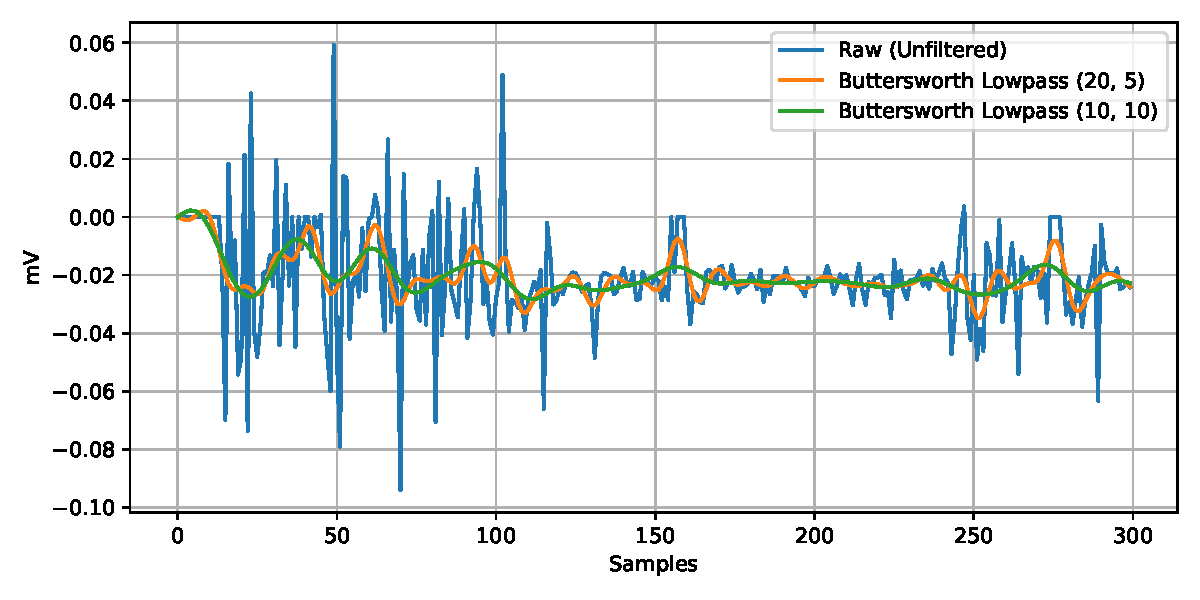
\includegraphics[width=0.99\textwidth]{lowpass.pdf}
\caption{Comparison of Buttersworth low-pass filters of different cutoff frequencies and orders.}
\label{fig:lowpass}
\end{center}
\end{figure}
\begin{figure}[H]
\begin{center}
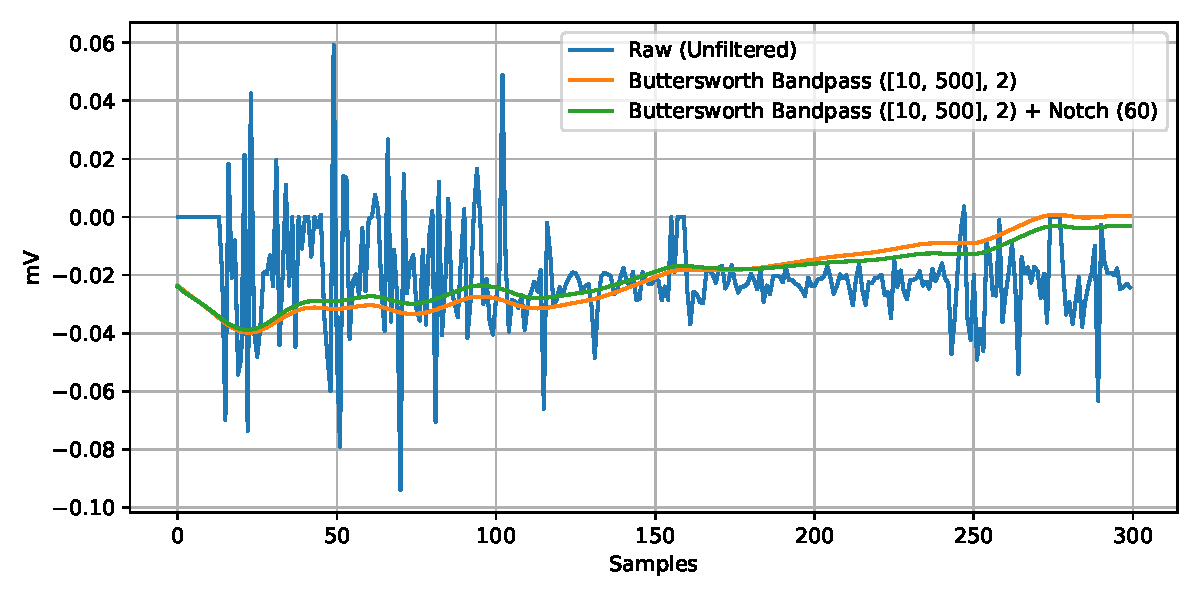
\includegraphics[width=0.99\textwidth]{bandpass.pdf}
\caption{Comparison of Buttersworth band-pass filters of different cutoff frequencies, orders and the usage of a Notch filter.}
\label{fig:bandpass}
\end{center}
\end{figure}

\subsubsection{Evaluation}

As can be seen in the figure, different configurations of pre-processing filters have a large impact on the resulting filtered sequence. 
It can be seen in figure \ref{fig:lowpass} that most of the change in amplitude exists in the low frequencies, and these are removed due to using a low-pass filter.
Furthermore, it can be seen that the intent of the signal is kept when a filter order of 5 is used, compared to a filter order of 10.
When comparing the two low-pass filters, it can be determined that using a cutoff frequency of $20Hz$ and a order of $5$ is a ideal for sEMG signals due to the amount of large frequencies in the recordings.
Alternatively, Buttersworth band-pass filters are tested in figure \ref{fig:bandpass},

\subsection{Dataset used for Training}

Due to the problems with the Motive motion capture software explained in section \ref{sec:motiveproblems}, it was determined that the main dataset for training the chosen methods would be based on dataset \cite{kinmusdataset} from the paper \cite{jarque2019}.
The dataset contains sections of sEMG data and kinematic movements of the hand.
These sections are labeled as either \textit{reaching}, \textit{manipulation} or \textit{releasing}.  
Due to the dataset containing data for regression and classification, it is possible to explore multiple methods of HMI's. 
The pre-processing step is not covered for the training dataset \cite{kinmusdataset}, as the dataset has been pre-processed using a 4th-order band-pass filter with a band of  $25$ to $500Hz$, then the data was subject to a 4th-order low-pass filter at $8 Hz$.
The main objective of these tests are to review and compare possible methods of regression \& Classification of sEMG data in order to determine the movements of the hand.

\section{Machine-Learning Intent Classification}
\label{sec:machine-learning}

Due to the dataset containing labels associated with movements of the hand, it is possible to use the dataset to train a intent prediction classifier.
As mentioned in the papers \cite{Batzianoulis2018} \& \cite{Yuki2023}, it is ideal to feature extract windows of the raw sEMG data.
The features \textit{Zero Crossing} \& \textit{Root Mean Square} are chosen as the features to extract for an intent classifier based on their heavy use as explained in \cite{Tech2015}.
Other features that could be chosen as an alternative would be variance \& mean-absolute-value.
Furthermore, the paper \cite{YanchaoWang2022} proposes that the Machine-Learning classifier LDA has the highest classification rate out of similar methods.
The paper \cite{Batzianoulis2018} proposes the use of the \gls{SVM} \gls{ML} method for intent classification.
Both types of classification will be explored and compared.

\subsection{Implementation}

In order to classify intent from sEMG muscle data, the data needs to be converted to feature space before it can be used as input to a machine learning algorithm.
For this, it was chosen based on state-of-the-art literature, that the feature extraction methods would be zero-crossing \& RMS.
The input channel for a single sEMG window was converted into a vector of zeros and ones for the zero-crossing features, where a one is set if the data crosses over the zero line.
Furthermore, the RMS for a window was calculated, and inserted to the end of the input vector. This effectively converts the 6 sEMG channels of a window size of $N$ into a feature vector of size $N+1$.
The feature-based inputs were extracted, and their movement labels were used as the target classification.
The resulting classification structure can be seen in Figure \ref{fig:mlclassifier}.

\begin{figure}[H]
\begin{center}
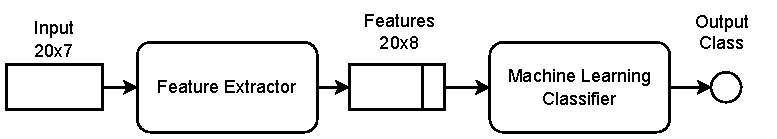
\includegraphics[width=0.99\textwidth]{MLClassifier.pdf}
\caption{The machine learning classifier setup with a feature extraction step.}
\label{fig:mlclassifier}
\end{center}
\end{figure}

The dataset of features and ground truths were then used as input for discriminant analysis, and SVM classifiers.
The purpose of \textbf{discriminant analysis} is to classify inputs into groups.
Discriminant analysis is a classical multivariate method of Supervised Learning, that takes a input set with their ground-truth classes and tries to maximize separation between these different classes.
The models assumes that data follows a Gaussian distribution. 
%TODO: True? Cite something for LDA QDA?
For this ML method, two types of discriminant analysis were tested on the dataset, namely LDA \& \gls{QDA}.
%Linear Discriminant Analysis (LDA) \& Quadratic Discriminant Analysis (QDA).
The main difference between LDA and QDA is that LDA makes the assumption that the covariance matrices of the classes are the same.
Equal covariance matrices will result in linear separations between classes.
QDA as an alternative does not assume this equal covariance, this results in a classifier that assumes quadratic separations between classes.
%The first method to test is the Linear Discriminant Analysis (LDA), and the second method was 
Just as discriminant analysis, SVM based methods are used to separate inputs into groups based on classes.
SVM is a robust supervised learning method that groups dataset classes.
SVM tries to maximize the width between classes by converting the input to a higher dimensional feature vector, and using this vector, the SVM algorithm is able to efficiently calculate a non-linear classification.
The feature space conversion is determined by the choice of SVM kernel in the algorithm.
For this ML method, 3 types of SVM classifiers were tested, a SVM using a Radial Basis Function (RBF) kernel, a SVM using a sigmoid Kernel and a NuSVM method with the RBF kernel and a parameter for the number of support vectors used.

\subsection{Tests \& Results}

The methods are tested on 50 sets of data that was not part of the training set.
The discriminant analysis methods can be seen in figure \ref{fig:lda_test}, with the average accuracy of the methods respectively being $61\%$ \& $55\%$ over the 50 tests.

\begin{figure}[H]
\begin{center}
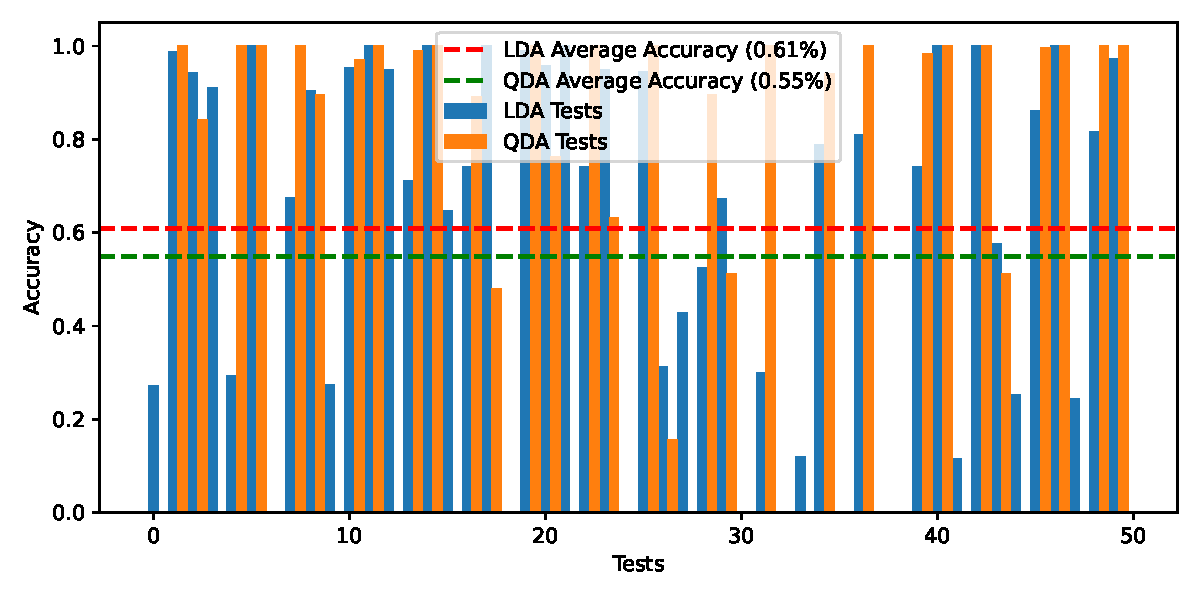
\includegraphics[width=0.99\textwidth]{lda_test.pdf}
\caption{Comparison of discriminant analysis methods (\gls{LDA}/\gls{QDA}) over 50 tests.}
\label{fig:lda_test}
\end{center}
\end{figure}
%TODO: Graphs does not show what bar is what type..

The \gls{SVM} methods can be seen in figure \ref{fig:svm_test}, with the average accuracy of the methods respectively being $54\%$, $56\%$ \& $59\%$ over the 50 tests.

\begin{figure}[H]
    \centering
    \begin{subfigure}[b]{1\textwidth}
        \centering
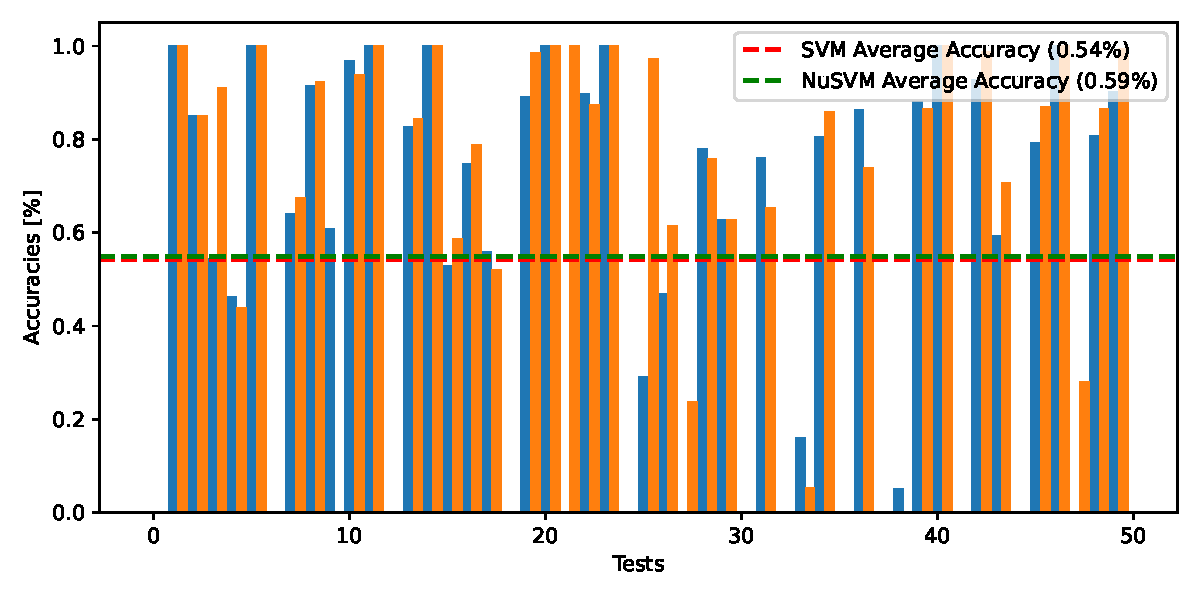
\includegraphics[width=0.99\textwidth]{svm_test.pdf}
%\caption{Comparison of Support Vector Machine Kernels (RBF/Sigmoid) over 50 tests.}
    \end{subfigure}
    \centering
    \begin{subfigure}[b]{1\textwidth}
        \centering
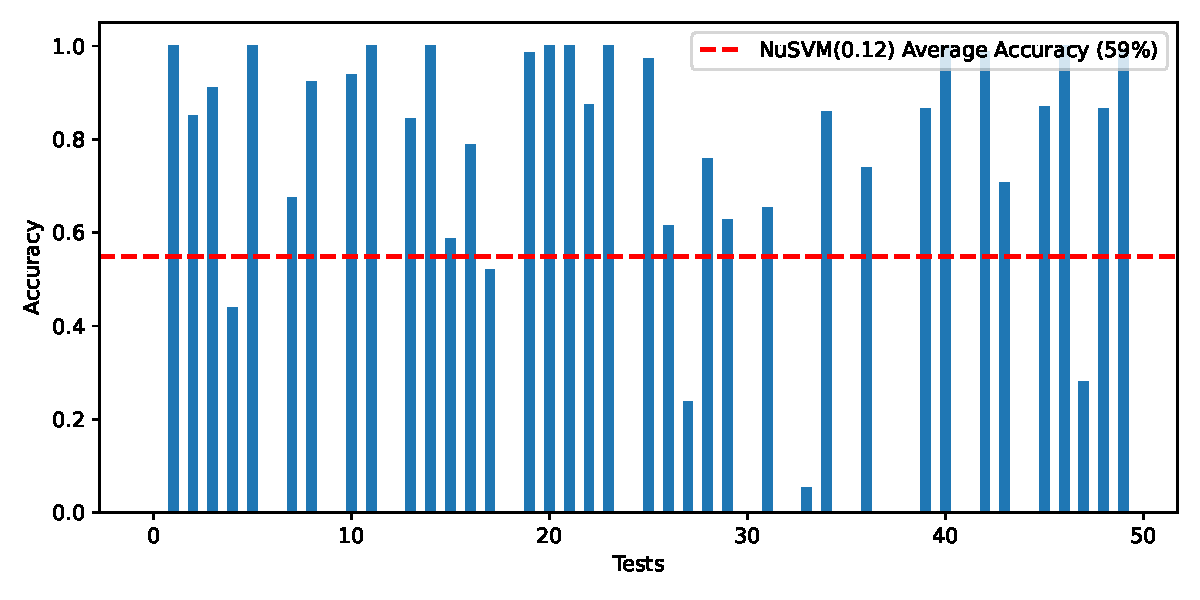
\includegraphics[width=0.99\textwidth]{nusvm_test.pdf}
    \end{subfigure}
    \caption{Comparison of \gls{SVM} Kernels \& parameters over 50 tests.}
\label{fig:svm_test}
\end{figure}
%TODO: Try another parameter for NuSVM so that the graph is more complete.

\subsection{Evaluation}

%TODO: GO through the graphs and talk about the results
The methods tested can be seen to have similar average accuracy of $\sim 60\%$ over 50 tests.
Because of this, it is difficult to choose a superior method without further analysis.
The choice of machine learning method depends on its overall classification rate over 50 tests, but it can also be important to rate the ML methods based on their inter-quantile values.
A full comparison of the machine learning methods can be seen in figure \ref{fig:classification_comparison}.

\begin{figure}[H]
\begin{center}
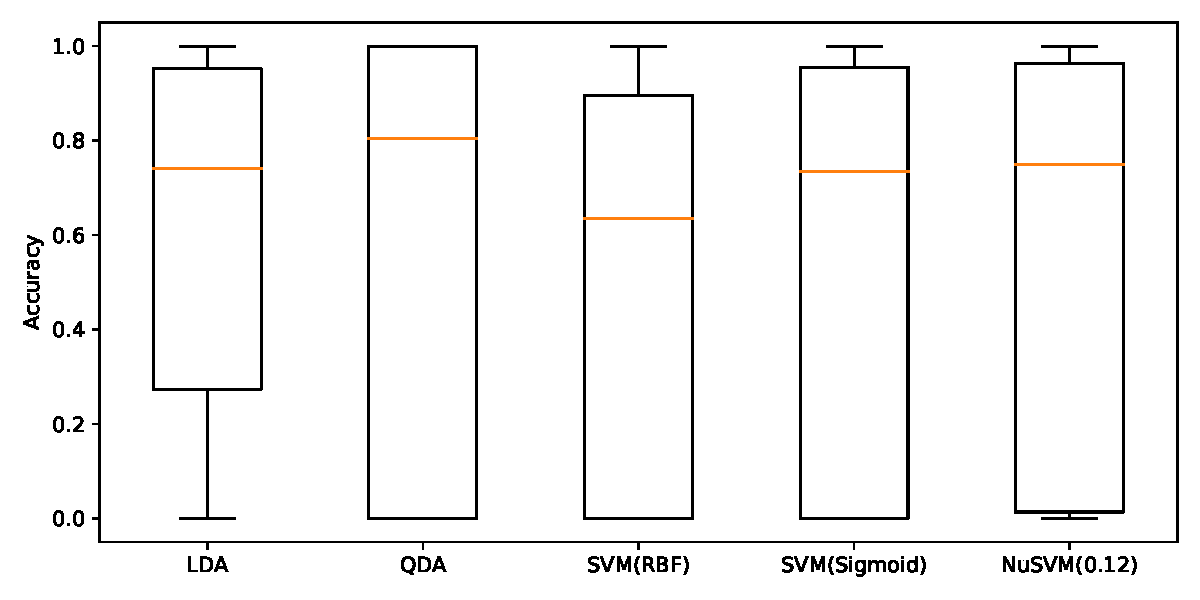
\includegraphics[width=0.99\textwidth]{classification_comparison.pdf}
\caption{Comparison of chosen classification methods based on accuracy over 50 tests.}
\label{fig:classification_comparison}
\end{center}
\end{figure}

It can be seen in the boxplot that most methods have a similar inter-quantile median, and fairly small whiskers.
In order to get a clearer comparison of methods, the relevant values have been compared in table \ref{tab:classification_comparison}.  

\begin{table}[H]
\begin{center}
\begin{tabular}{ |l|c|c|c| } 
 \hline
 ML Method & avg-accuracy [\%] & Inter-quantile Median & Inter-quantile Range \\ 
 \hline
 LDA & \textbf{61\%}           & 0.741705 & \textbf{0.679410} \\ 
 QDA & 55\%           & \textbf{0.803432} & 1.000000 \\ 
 SVM (RBF) & 54\%     & 0.634426 & 0.895688 \\ 
 SVM (Sigmoid) & 56\% & 0.735050 & 0.955580 \\ 
 NuSVM (0.12) & 59\%  & 0.749436 & 0.950715 \\ 
 \hline
\end{tabular}
\caption{Comparison of relevant classification parameters for the chosen methods. The best performing parameters have been highlighted.}
\label{tab:classification_comparison}
\end{center}
\end{table}
%         label  lower_whisker  lower_quartile    median  upper_quartile  upper_whisker
% 0          LDA             0.0        0.273173  0.741705        0.952582            1.0
% 1          QDA             0.0        0.000000  0.803432        1.000000            1.0
% 2      SVM(RBF)            0.0        0.000000  0.634426        0.895688            1.0
% 3  SVM(Sigmoid)            0.0        0.000000  0.735050        0.955580            1.0
% 4   NuSVM(0.12)            0.0        0.013333  0.749436        0.964048            1.0

% Inter-Quantile range
% 0    0.679410
% 1    1.000000
% 2    0.895688
% 3    0.955580
% 4    0.950715

The relevant parameters in the table makes it possible to identify the most suitable method for intent classification.
It can be seen that LDA has the overall best accuracy of all the methods of $61\%$, and the overall worst performing method is SVM (RBF).
By denoting the median and the range of the inter-quantile section of the boxplots, we can further elaborate on the accuracy of the 50 tests.
% LDA
LDA has the best average accuracy, and it also has the smallest inter-quantile range, indicating that LDA perform well across tests with a robustness to outlier tests. 
% QDA
It can be seen that QDA performs best according to the inter-quantile median, but QDA is also the method that has the largest inter-quantile range indicating that QDA is not very robust to outlier tests.
% NuSVM
An alternative to the discriminant analysis methods, it can be seen that the NuSVM method with a number of support vectors denoted by $0.12$.
NuSVM has the second best average accuracy, the second best inter-quantile median \& the third lowest inter-quantile range.
% Conclusion:
From the table \ref{tab:classification_comparison}, it becomes apparent that none of the methods have ideal performance, but that the LDA method is the best method for intent classification.
This result is similar to the conclusion in paper \cite{KeunTaeKim2021}.
% Eval on feature extraction
The resulting performance metrics of the ML methods are dependent on the chosen feature extraction techniques used.
Zero crossing and MSE features can be used for the classifiers and provide insight into what parameters are important when working with sEMG data.

%\newpage
%TODO: Experiment with no line breaks, is it bad?
\section{Neural Network Movement Regression}
\label{sec:regression}

As an alternative to intent classification, it was determined that the dataset would be ideal for regression of the joint angles of the fingers.
Several methods is explored, both window and recurrent based networks are tested.


\subsection{Windowed Convolutional Neural Network}

\subsubsection{Implementation}
% TODO: Why did my network end up looking like this?

%TODO: WHY CHOOSE A CNN? SELL IT LIKE A CAR!
The sEMG data used as input for regression networks is complex.
The sequences of muscle activity needs to be understood by the proposed method and produced into a an output.
A network type that is ideal to understand complex meaning in, 3-dimensionary inputs is a CNN network.
%A CNN is an alternative to a MLP network that is similar in functionality is a Convoluted Neural Network (CNN).
A CNN consists of a set of Convolution Layers that deforms inputs to abstract convolution features.
The structure is considered sparsely connected due to the convolution layers are only receiving a subset of the previous convolution features.
The feature conversion is ideal when a network needs to become robust and needs to recognize larger concepts in the input.
This functionality is especially used when the input data takes the shape of a matrix.
Once the input is convoluted to a chosen feature abstraction, it is given to a MLP structure trained to convert the convolution features into a usable output.
%TODO: needs sources for this stuff?
%TODO: Go back and see what papers uses CNN's
CNN networks have no build-in time-based functionality, they receive a set of inputs and produce an output.
It is possible however to represent time if the input is given in segments consisting of multiple time-frames.
Because of this, the sEMG muscle activity from the dataset is segmented into windows of a desired size, the output angles that the network should do regression towards are then chosen to be the first angle after the window.
%TODO: Images of these for better clarity!!!!
A CNN network can be used in the field of sEMG processing due to the convolution layer's ability to learn abstract formations of the sEMG data.
The network would be able to identify patterns in sEMG data and correlate them to an appropriate output.
%TODO: formations? another word?
The CNN network structure seen in figure \ref{fig:cnn_structure}.

\begin{figure}[H]
\begin{center}
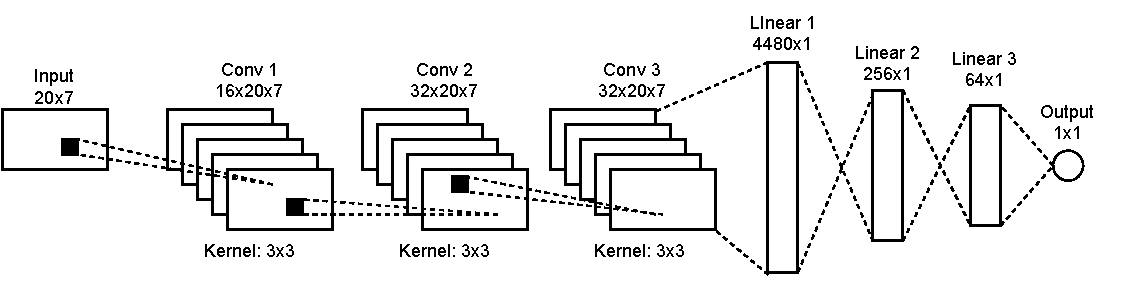
\includegraphics[width=0.99\textwidth]{cnnstructure.drawio.pdf}
\caption{The chosen CNN network structure, consisting of 3 Convolution Layers and 3 Linear layers. Network input is a window of sEMG recordings, with the purpose of regression of a finger joint angle.}
\label{fig:cnn_structure}
\end{center}
\end{figure}
%TODO: The 20 in this case refers to N samples! if i want something else than 20, change the image!

As visualized in the figure, the CNN network consists of 3 Convolution layers followed by 3 MLP layers.
The network is designed through manual hyper-parameter tuning based on validation error reduction of the model.
The structure of the network is designed to be simple with a small amount of convolutions without pooling due to the small input size.
The Convolution layers extract features up to a size of 32 using a convolution kernel with a size of [$3, 3$].
The convolution features are then flattened, to a size of $4480$, and processed by 3 hidden layers convert the convolution output into a regression prediction.
%A CNN is trained on the network, using a window size of 40 samples were used.
%TODO: Give example of a state-of-the-art paper CNN as an alternative to mine!!!
The CNN network is trained to do regression of joint angles of the hand, because of this, the loss function is determined to be MSE loss.
The network is trained using an Adam optimizer with a learning rate of $1\text{e}^{-4}$.
A subset of the dataset is split into a test and a validation set, and windows are extracted correlating input and output.
The output is normalized, and the input/output sets are shuffled before training takes place.


\subsubsection{Tests \& Results}

%In order to test the CNN network and assess its performance, the training MSE loss can be seen in figure \ref{fig:cnntrainvalid}.
%TODO: Make sure this graph is explained properly and is the actual image

%\begin{figure}[H]
%\begin{center}
%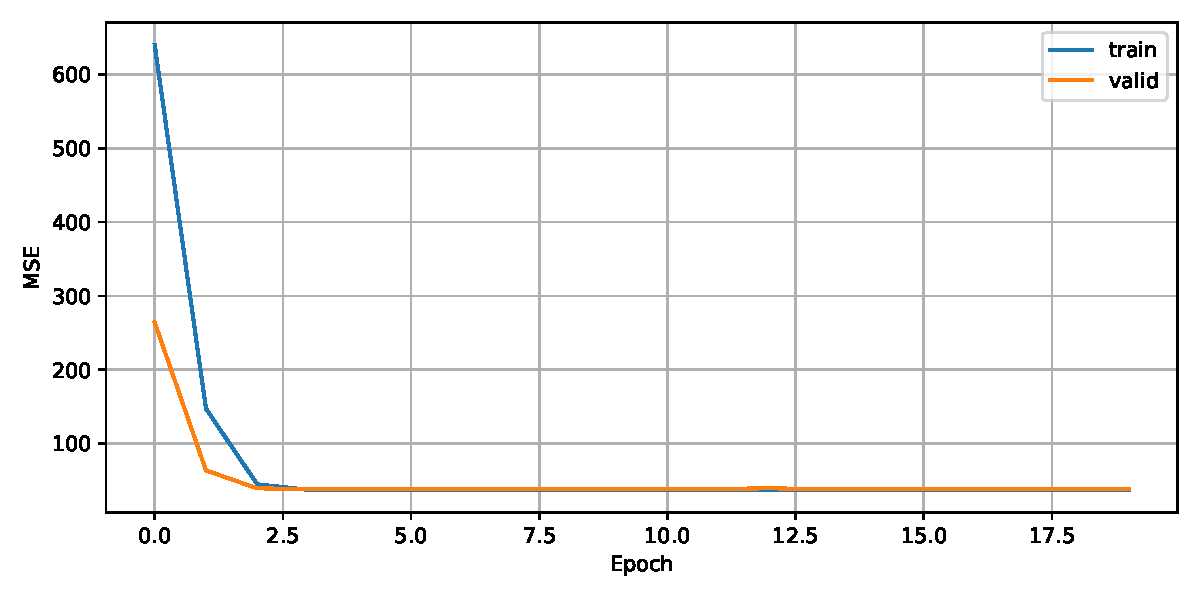
\includegraphics[width=0.8\textwidth]{cnn_trainvalid.pdf}
%\caption{The Train and Validation MSE loss during training of the CNN network method.}
%\label{fig:cnntrainvalid}
%\end{center}
%\end{figure}
%
%TODO: Maybe remove this
The CNN network is trained with a batch size of 8 over 20 epochs, with the resulting MSE loss settling at $\sim 34$ after 3 epochs.
50 sets of regressions that have not been trained on are taken from the dataset for testing.
The errors of the dataset are plotted, as can be seen in figure \ref{fig:cnntest}.

\begin{figure}[H]
\begin{center}
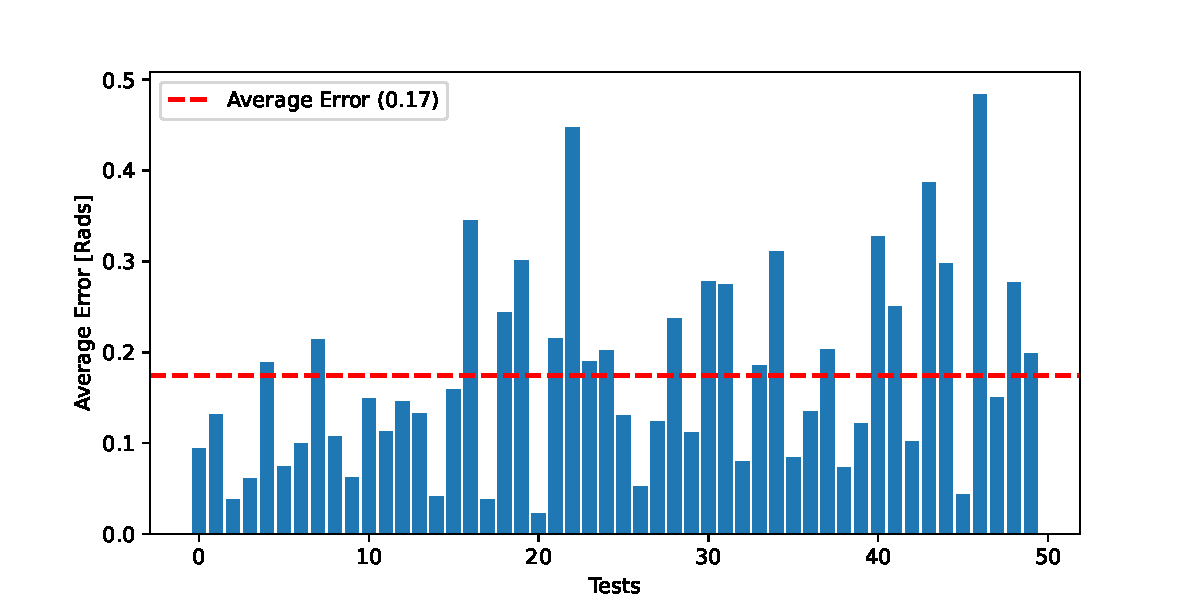
\includegraphics[width=0.99\textwidth]{cnn50test.pdf}
\caption{The errors of 50 regressions using the CNN network.}
\label{fig:cnntest}
\end{center}
\end{figure}
%TODO: What i need to do:
% Pull out 50 sets of data, do regression using my cnn model, plot their average errors in a barplot!
% This method will be my main regression test!


\subsubsection{Evaluation}

The CNN network is able to be trained on the dataset with a validation set MSE loss of $34$.
The errors of the 50 test regressions in figure \ref{fig:cnntest} show that a fairly large average regression error of $0.17$ Radians exists in the test regressions, and that the average error is skewed upwards due to some outlier tests having large average errors up to $0.3$ Radians.
%TODO: Get the max error!

%TODO: Maybe do a average error boxplot too?


\subsection{Recurrent Neural Network Regression}

%TODO: Why did my network end up looking like this?
Due to sEMG data being time-based, Recurrent network types are ideal for regression predictions.
RNN networks are similar to MLP's with the main difference being that a RNN has hidden feedback  memory state that is derived from earlier inputs.
This functionality makes RNN networks ideal for concurrent, time-based systems where a sequential input distribution needs to be converted to a output regression.  
%TODO: Alternative to concurrent -> i want something that explains a set of data in a graph!
Another use case of RNN-based regression systems are systems where response time is critical.
The RNN network does not use a window of data, it converts the input of the current time frame, and the feedback of the previous time frame into a prediction.
Because of the hidden memory, a RNN network has a quicker response time than a window-based network.
The RNN network structure designed to predict regression of finger movements from sEMG data can be seen in figure \ref{fig:rnn_structure}.
The network is designed through manual hyper-parameter tuning based on validation error reduction of the model.

%TODO: This one sounds nice, can it be integrated?
%The recurrent feedback loop correlates previous predictions with future predictions, allowing the network to approximate regressions per time frame.


\begin{figure}[H]
\begin{center}
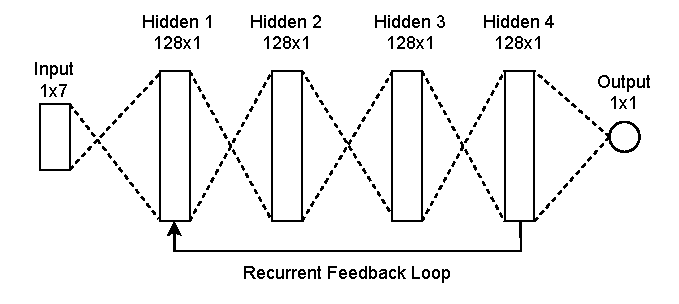
\includegraphics[width=0.8\textwidth]{rnnstructure.pdf}
\caption{The chosen RNN network structure, consisting of a input layer, 4 hidden layers with a recurrent feedback loop, and a output layer.}
\label{fig:rnn_structure}
\end{center}
\end{figure}

\subsubsection{Tests \& Results}

The RNN network is trained on the dataset \cite{kinmusdataset}, in a similar way as the CNN network, with the purpose of approximating finger angle regressions per time frame.
The RNN network is trained with a batch size of 8, with the  MSE loss function and the Adam optimizer with a learning rate of $1\text{e}^{-2}$.
In order to test the network, a random set of 50 regressions that have not been trained on are taken from the dataset.
The average errors of each regression test is plotted, as can be seen in figure \ref{fig:rnntest}.

\begin{figure}[H]
\begin{center}
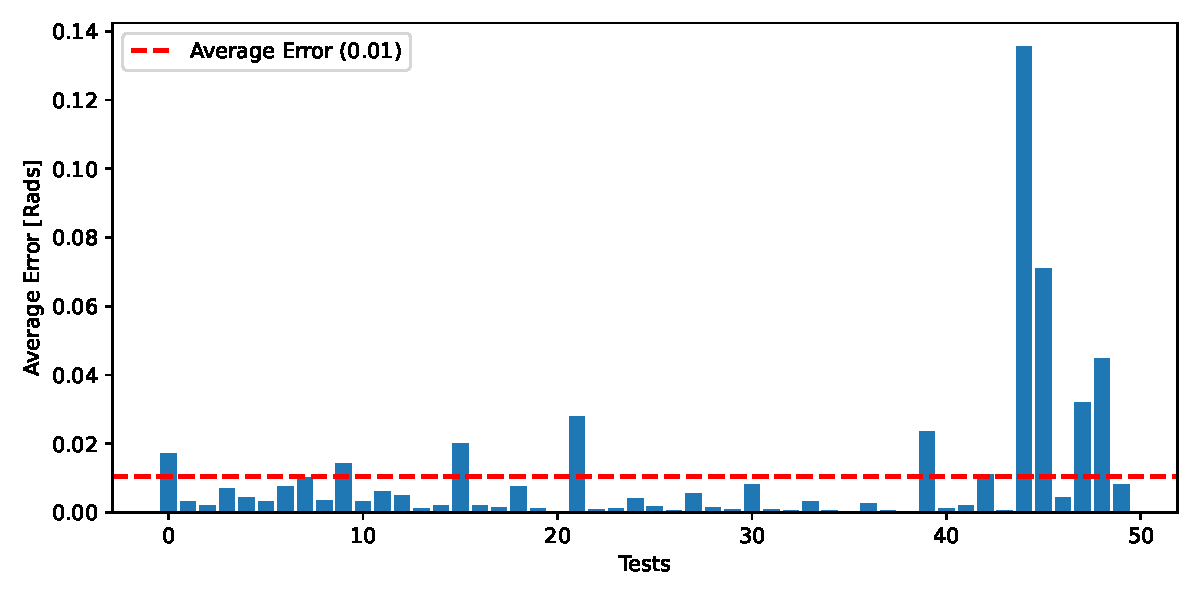
\includegraphics[width=0.99\textwidth]{rnn50test.pdf}
\caption{The errors of 50 regression tests using the RNN network.}
\label{fig:rnntest}
\end{center}
\end{figure}

\newpage
\subsection{Evaluation of Regression Methods}

%As can be seen in figure \ref{fig:cnntrainvalid}, the CNN network is able to be trained on the dataset with a fairly low MSE loss.  
The errors of the 50 test regressions in with the different models can be seen in figure \ref{fig:regression_comp}.

\begin{figure}[h]
\begin{center}
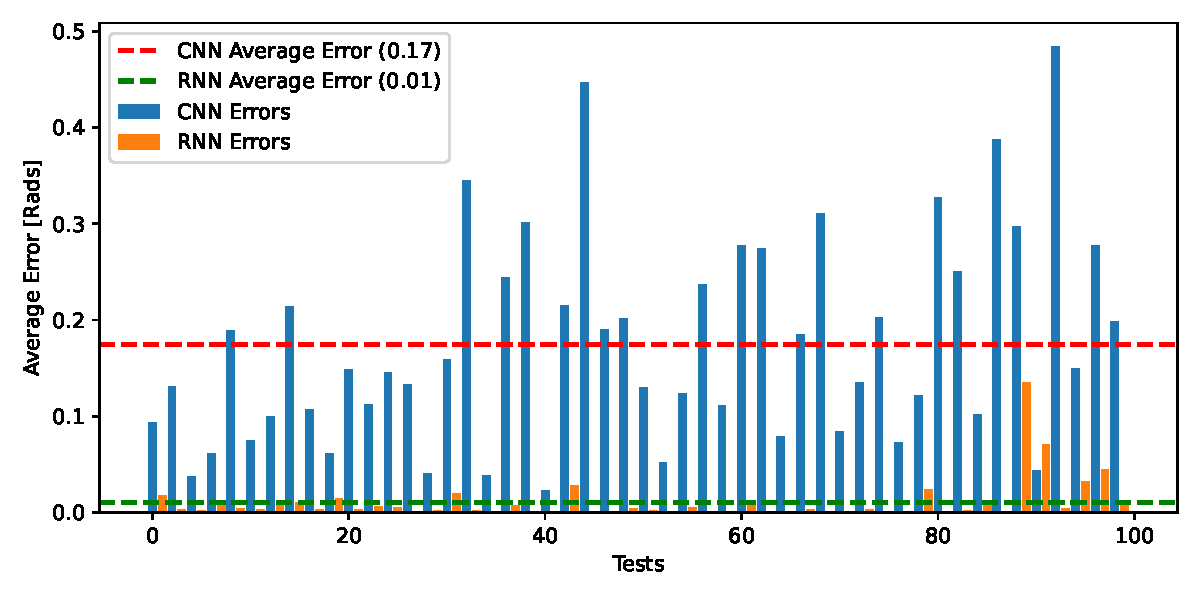
\includegraphics[width=0.99\textwidth]{regression_comparison.pdf}
\caption{Comparison of Windowed CNN and RNN regression methods.}
\label{fig:regression_comp}
\end{center}
\end{figure}

The figure clearly shows that there is a large difference in window-based and recurrent network types.
The CNN shows a average test error of $0.17$ Radians, while the RNN network has a average test error of $0.01$ Radians. 
The reason for the large error in the CNN network test is unclear.
One of the reasons the CNN network is unable to accurately learn regression could be because of the pre-processing done in the dataset.
Alternatively, the network is unable to learn because of the window size. This would make sense since the RNN network with a really low error is able to learn to do regression, as it is not limited by a arbitrary window of input.

It becomes apparent that teaching a neural network to do regression of finger joints is a complicated task.
Because of this, the tests propose that it is ideal to use a type of Recurrent Network for regression.

%TODO: Maybe do a average error boxplot too?

%TODO: Some introduction and explanation of RNN and LSTM types of networks.
%TODO: Go back and see what papers uses these.

%\subsubsection{Long-Short-Term-Memory Recurrent Neural Networks}
%TODO: Create this if you have the time..
%A variant of a RNN can contain a special kind of hidden memory called Long Short Term Memory (LSTM).
%a LSTM uses gates as a way of containing a memory.

%\section{Comparison of Regression-based Networks}

%\subsection{Feature-Based Multi Layer Perceptron Network}

%Neural Networks are widely used in the field of AI.
%One type of widely used neural network is a fully-connected Multi-Layer Perceptron (MLP) Network.
%The MLP network is popular due to its structure and training capabilities.
%A MLP consists of layers of weighted activation functions where each activation function in a layer recieves the entire previous layer's output summed up as input.
%Due to the structure of a MLP, the network is capable of recieving a set of inputs and be trained to approximate a n'th degree polynomial function that relates the given inputs and outputs.
%The network is trained by updating the individual weights through backpropagation with the predicted output and a ground-truth output.
%The MLP network could be used to predict the relation between muscle activity and finger movements.

%In order to initially test the the dataset, a simple MLP network will be trained as a baseline for performance, and for testing the general applicability of window-based networks.


%TODO: Explain the software i made to clearn motive!
%TODO: Explain and showcase some pre-processing filters mentioned by other papers!
%TODO: Maybe here, maybe in methodology: Show how the gt angles are calculated too..

\newpage
\section{Simulated Prosthetic Hand}
\label{sec:simtest}

\subsection{Useability of the Simulated Prosthetic Hand}
%\subsection{Anatomical Assessment and Maneuverability}

Access to existing prosthetic hand simulations proved to be impossible to access and use.
they are either unavailable because their associated products have been discontinued or locked behind a pay-to-access barrier where you have to pay to receive a real prosthetic.
Due to non-availability of prosthetic hand simulations, it was chosen that through this thesis, a open source prosthetic hand needed to be created for testing of the algorithms developed as part of this project.
The creation of a prosthetic hand simulation can be seen in section \ref{sec:prost_sim}.
The prosthetic hand was designed to be as anatomically similar as a real hand as possible.
This was done in order to accurately simulate the movement of a real hand, and because of it, allow users to test and validate control methods on a simulation before needing to construct a real prosthetic.
The usability and dynamic movement of the simulated prosthetic hand needs to be assessed.
This is important because the usability of a prosthetic hand has a large impact on rehabilitation for the end-user.

\subsection{Method}
In order to test the usability and dynamic movement of the simulated prosthetic hand, the hand was tasked with achieving the end-poses of the most used day-to-day grips.
These grips were explained in section \ref{sec:dataset} table \ref{tab:grips}, namely the \textit{Pulp pinch}, \textit{Lateral pinch}, \textit{Five-Finger pinch} \& \textit{Diagonal Volar grip (Power grip)}.
In order to pose the simulated hand, the interface created in ROS2 was used to send kinematic configurations to the hand simulation.

\subsection{Test \& Results}

The hand was posed into all 4 day-to-day grip configurations for visual assessment.
The resulting configurations of the hand can be seen in figure  \ref{fig:hand_pose_test}.
The software used to pose the hand simulation can be seen in appendix \ref{appendix:roscontrol} 

%\begin{figure}[H]
\begin{figure}
    \centering
    \begin{subfigure}[b]{0.49\textwidth}
        \centering
        %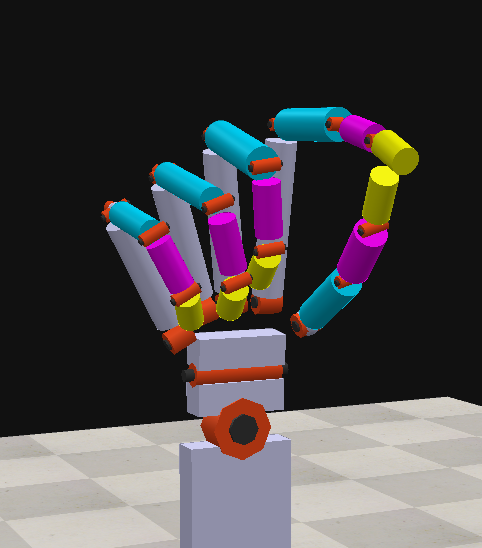
\includegraphics[width=\textwidth]{pulppinch_grip.png}
        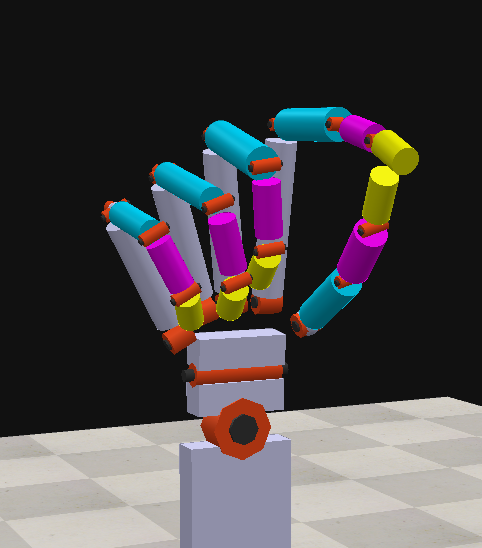
\includegraphics[height=8cm]{pulppinch_grip.png}
        \caption{Pulp pinch}
    \end{subfigure}
    \hfill
    \centering
    \begin{subfigure}[b]{0.49\textwidth}
        \centering
        %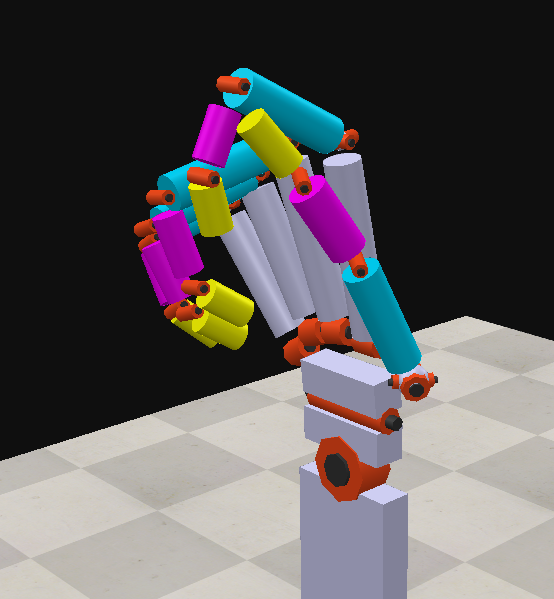
\includegraphics[width=\textwidth]{lateralpinch_grip.png}
        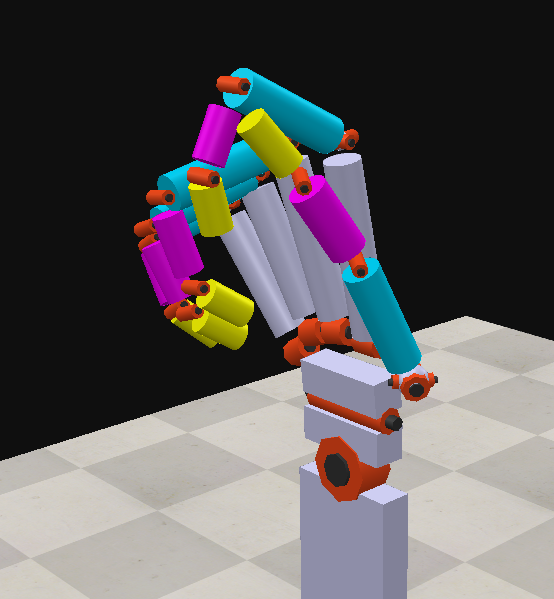
\includegraphics[height=8cm]{lateralpinch_grip.png}
        \caption{Lateral pinch}
    \end{subfigure}
    \hfill
    \begin{subfigure}[b]{0.49\textwidth}
        \centering
        %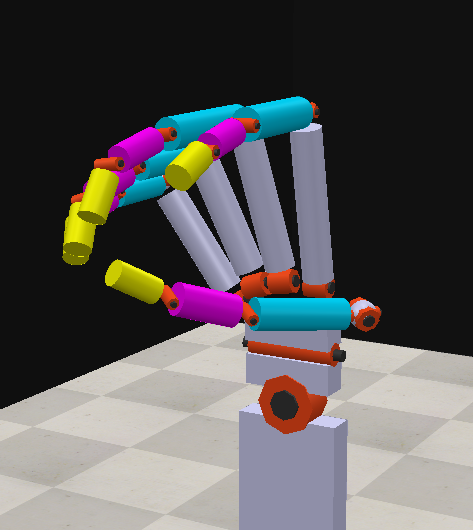
\includegraphics[width=\textwidth]{fivefingerpinch_grip.png}
        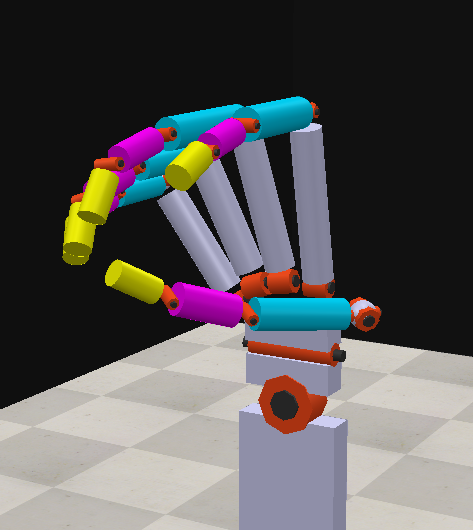
\includegraphics[height=8cm]{fivefingerpinch_grip.png}
        \caption{Five-Finger pinch}
    \end{subfigure}
    \hfill
    \begin{subfigure}[b]{0.49\textwidth}
        \centering
        %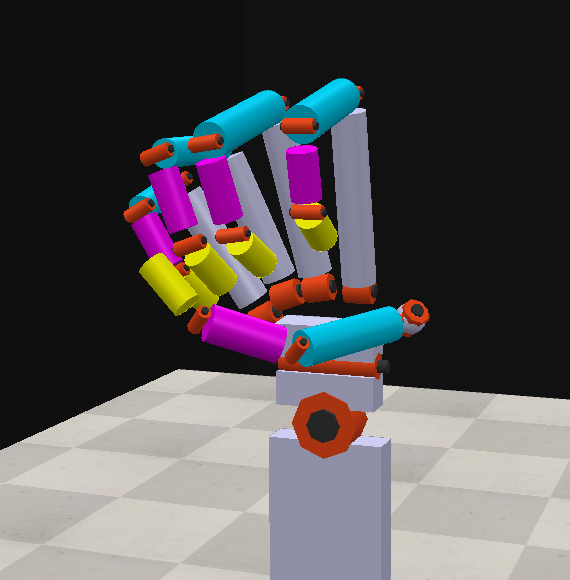
\includegraphics[width=\textwidth]{power_grip.png}
        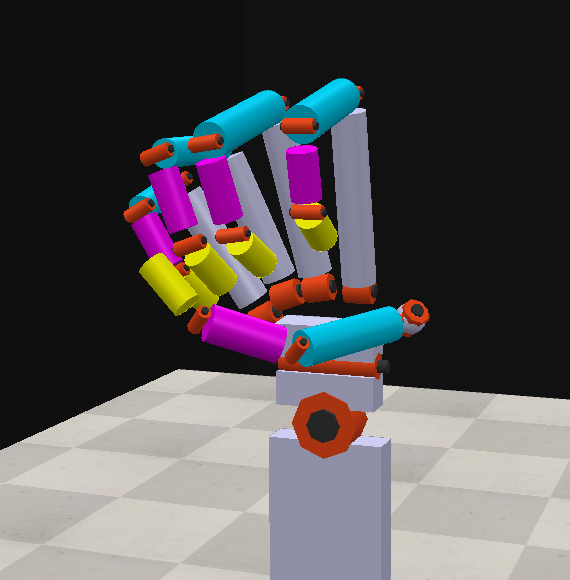
\includegraphics[height=8cm]{power_grip.png}
        \caption{Diagonal Volar grip (Power grip)}
    \end{subfigure}
    \caption{The four most used day-to-day poses, tested in a hand prosthetic simulation.}
    \label{fig:hand_pose_test}
\end{figure}


%TODO: Needs to be a figure of figures!
%\begin{figure}[h]
%\begin{center}
%\includegraphics[width=0.8\textwidth]{example-image-a}
%\caption{Example figure text}
%\end{center}
%\end{figure}

\subsection{Evaluation}

Based on a visual assessment of figure \ref{fig:hand_pose_test}, it can be concluded that the prosthetic hand is able to be posed similarly to the real-life reference.
The ROS2 interface created for the simulation allows for easy manipulation of the joint rotations, and because of this, achieving different poses becomes easy to do.
The hand simulation is able to achieve a wide range of motion because of its design and its ability to mimic the anatomy of the real hand.
From this it can be concluded that the prosthetic hand is proportionally correct and thus also allows for accurate posing, applicable in different day-to-day scenarios.

%\newpage

% this thing is not possible..
% should i have a explanation for not doing it?
%\subsection{Posing based on Network Output}
%
%%TODO: More here..
%As a result of testing different network types and their applicability for creating suitable motor control output for a prosthetic hand, it would be ideal to test the network output on the prosthetic simulation.
%For full video see appendix ??.
%TODO: Insert appendix here



%TODO: see Zhaolong2021 (page 10) for example of how to compare MSE for different neuron amounts, even for multiple subjects!



%TODO: Show graphs of different filters!
%TODO: Talk about what filters are and how they affect incoming signals, what type to use against what noise etc. 

\end{document}

\documentclass[../main.tex]{subfiles}
\graphicspath{{\subfix{../src/}}}


\begin{document}
\section{Discussion}

The main purpose of this thesis is to research and experiment with state-of-the-art sEMG-based human-machine-interfaces for development of prosthetic devices.
The experimentation is mainly done with the focus of identifying and modeling the intent \& movement of the fingers.
% Mention gazebo and copelliasim problems
During the development of this thesis, several problems occurred with the chaise of simulation tools.
The initial chosen simulation software was the Gazebo \cite{gazebo} due to its close integration with ROS2 \cite{ros2}, and its use in modern robotics simulation tasks.
After a lot of long-term problems and complications caused by the chosen software, a decision to switch to CoppeliaSim \cite{coppeliasim} was made.
The change to CoppeliaSim solved a lot of the problems caused by Gazebo, the setup of the simulation and development of the kinematics became much clearer.
Furthermore, setting up the controller of the prosthetic could be done using the build-in ROS2 communication.
%TODO: Problems with motive
%      Data unreliability
%      having to make my own methods to clean data
%      Unable to create a proper dataset with own methods
%      Unable to have multiple people in the dataset due to extensive clearning
Another problem had a large impact on the development of this thesis.
In order to capture the movements of the fingers for the dataset, the product Motive Motion Capture Setup \cite{motive} was chosen, due to recommendation, availability and its use in state-of-the-art industry motion capture.
The Motive setup consists of a camera rig designed to locate 3D markers in the scene.
As a recording target, a glove was fitted with 3D markers.
This was done in order to record the kinematic movements of the hand, a glove is fitted with 3D markers at the joints of the fingers.
%so that it would be possible to calculate the angles between the 3D markers.
The main problem is that the setup is designed to capture large objects such as full-body tracking suits and larger static objects.
Because of this, the 3D optimization algorithms used by the cameras has a tendency to remove markers that are close. 
This would cause the 3D markers of adjacent fingers to be combined into a single marker.
The only way to solve this is to reduce the amount of markers on the glove.
Furthermore, the 3D marker labeling is unreliable.
The markers are shifting in labels if they disappear for a few frames at a time.
This problem scaled with the length of the recording session, a 15 second recording of 7 markers would be recorded as $100+$ labels in the resulting tracker output.
In addition to the tracking being unreliable, the Motive software is unable to provide an effective label correction tool.
Label rendering \& correction tools is developed as part of this thesis, and is used to clean up a subset of the recorded dataset.
Due to the extensive work needed to record and clean the movements of the hand, it became impossible to create a dataset large enough to train models on, and to create a general purpose dataset with recordings from multiple people. 
The time-consuming process of creating a simulated prosthetic and recording a dataset resulted in some of the goals of this thesis as explained in section \ref{sec:goals} to not be fulfilled.
It was not possible to fully test the simulated prosthetic device with real-time predictions from a model. 
% if i had the time: compared kinematic output with control of the sim hand.
Furthermore, it was not possible to fully test different pre-processing methods and their differences when used for training a model.

%TODO: Explain that actual angle calculation was not done for recorded markers.

\textbf{Classification Tests}\\
% It would have been nice to test different types of feature extraction methods for classification.
Multiple different machine learning methods is tested in section  \ref{sec:machine-learning}
The data is converted to a feature space set consisting of zero-crossing and MSE, and is then used as input to a machine learning algorithm to create a lower-arm intent classifier.
The accuracy of the resulting classifiers could have been improved, if more types of feature extractions had been tested.
Furthermore, different types of machine learning classifiers and network based classifiers could have been tested in order to improve classification accuracy.

\textbf{Regression Tests}\\
Different regression network models were trained to do regression of finger joint angles. These tests can be seen in section \ref{sec:regression}.
Window based regression network methods were compared to recurrent network based methods.
The window based regression has a large error, and it is unclear what the exact cause is.
The large error could be result of using an incorrect size of window, or the result of the training data not being optimal for training.
The error could also be the result of the training parameters used, and it might have been solved by extensive parameter tuning.
The use of a recurrent network proved to have very accurate results for regression of finger angles.

\textbf{Hand Simulation Tests}\\
The simulated hand created in CoppeliaSim \cite{coppeliasim} is tested in section \ref{sec:simtest}.
The hand is designed to be anatomically proportional to a real hand, with the same amount of degree of freedom as its real counterpart.
The tests were created to assess the simulated prosthetic hand's ability to be manipulated and its ability to perform anatomically correct poses.
The hand was manipulated to the 4 most used day-to-day grip types with great precision by a visual assessment.
The main problem with the hand simulation is that it was not possible to test its performance using the output of a regression model as a controller.
This was not possible due to the created dataset.



%TODO: Tests not being too good, explain its due to dataset problems,
% Explain more time could have been used on methods fine tuning and experimentation, if there had been no problems with dataset creation.

%TODO: CNN network seems to approximate the median of all the ground truth regression angles.

% Results are liable to parameter tuning

% if i had the time: compared kinematic output with control of the sim hand.

\end{document}

\documentclass[../main.tex]{subfiles}
\graphicspath{{\subfix{../src/}}}


\begin{document}
\section{Conclusion}

This thesis is developed with the purose of researching \& designing a state-of-the-art sEMG-based HMI for a simulated prosthetic hand.
% Chosen hardware stuff explained 
During the development of this thesis, a controllable prosthetic hand was developed in the simulation tool CoppeliaSim \cite{coppeliasim}, that is able to be controlled by the commonly used robotics communication software ROS2 \cite{ros2}.
The prosthetic hand is designed to have anatomically correct porpotions, with anatomically correct joints that allows the simulation to act and be controlled with similar movements as a real hand. 
The simulation is created with the purpose of providing an easy-to-use, freely available, advanced prosthetics simulation for others to use, modify and develop with. 
Another purpose of this thesis is to research and test state-of-the-art HMI techniques in the field of AI and ML, in order to compare and test different methods of converting sEMG based muscle activity into a useable controller scheme for a prosthetics device.
This thesis tests two different areas of HMI interfaces, ML based lower-arm intent classification and AI based finger movement regression.
Different models in each area are tested and compared, based on reccomendations of state-of-the-art
literature, in order to determine what models are ideal for the control of a prosthetic hand.
% in debth of classification
Several different ML models were trained and compared in section \ref{sec:machine-learning}.
All models were trained on feature-space converted sEMG data.
Based on the tests and comparison of the classification accuracy table \ref{tab:classification_comparison}, it can be seen that the Linear Discriminant Analysis (LDA) performs best in average accuracy of $0.61\%$ and interquantile range of $0.679\%$.
It can also be seen, and that QDA performs best in the interquantile median with a value of $0.803\%$.
From this, the LDA machine learning algorithm is proposed to be best at intent classification of the lower-arm.
% in debth of regression
As an alternative to intent classification, different AI models designed to do regression of finger movements were trained and compared in section \ref{sec:regression}.
Based on the regression comparison in figure \ref{fig:regression_comparison}, it can be seen that Recurrent methods perform best compared to window based methods.
This can be seen when comparing the average error in 50 tests, the CNN network has an average error of $0.17$ Radians per test, where the RNN network has a low average error of $0.01$ Radians.
% in debth of dataset creation proposal
The designed models are trained and tested using a freely available dataset \cite{kinmus}.
This was done due to problems with the chosen Motive Motion Capture setup, these problems were reduced by the implementation of a rendering and cleaning software explained in section \ref{sec:motivecleaner}.
%TODO: CREATE THIS SECTION
Using this implemented software, it is possible to fixing wrong labels and removing labels all together, compared to the building functionality in Motive.
%This software makes fixing wrong labels and removing labels all together possible, compared to the building functionality in Motive.
With this implemented software, it was possible to clean a small subset of recorded data, but it was not possible to create a full dataset of multiple people.
% with cleaning of data 


% TODO: Take it further and go into detail on my goals and what worked and what didnt

\newpage
\subsection{Future Work}

Due to the problems encountered with the chosen software in this thesis, some parts of the motivation goals in section \ref{sec:goals} were not possible to explore.
Had it been easier to create a custom dataset, preferably with recordings from multiple people, it would have been possible to explore further combination of the created prosthetic and the trained models.

Further testing, exploring, and controllability of a trained model in a simulated environment could also have been explored.
This could be done in real-time, where a trained model could be used to convert live sEMG recordings into movemements for the simulated prosthetic, allowing the test person to manipulate the simulated environment in real time.
The work done in this thesis mainly explores two different areas of prosthetic controllers, classification based and regression based.
Had a large dataset created specificly for the purpose of this thesis been created, it would be ideal to test the applicability of combining methods and by doing so, explore possible controller schemes that combines the individual movement of regression models and the robustnes of intent classification.  

% TODO: Go back to problem and create some pointers to what is applicable based on my work

\end{document}


% TODO: Refrences

\include{content/appendices.tex}

\end{document}
